\documentclass{article}
\usepackage[utf8]{inputenc}
\usepackage[spanish]{babel}
\usepackage{graphicx}
\graphicspath{ {images/} }

\begin{document}

\begin{titlepage}
    \begin{center}
        \vspace*{1cm}
            
        \Huge
        \textbf{Diseño y planeacion}
            
        \vspace{0.5cm}
        \LARGE
            
        \vspace{1.5cm}
            
        \textbf{Danier Santiago Ortega Restrepo}\\
        \textbf{c.c.1036681098}\\
        
        \textbf{Jose Manuel Rivera Villa}\\
        \textbf{c.c.1000860503}
            
        \vfill
            
        \vspace{0.8cm}
            
        \Large
        Despartamento de Ingeniería Electrónica y Telecomunicaciones\\
        Universidad de Antioquia\\
        Medellín\\
       Octubre de 2021
            
    \end{center}
\end{titlepage}

\newpage
\tableofcontents
\section{Modelamiento de clases}
\subsection{Clase Personaje}
Esta clase esta definida como el manejo de los movimientos del personaje, estructura del personaje principal, animaciones con la interaccion del mapa, por ejemplo las muertes, saltos y movimientos.
\subsection{Clase Plataforma}
Esta clase contiene el modelamiento de las plataformas sobre las cuales el personaje se podra mover y ubicar en el trascurso del juego, tendra diferentes atributos para crear diferentes tipos y tamaños de plataformas, para ubicarlas dentro del mapa.
\subsection{Clase Mecanica Principal}
Dentro de esta clase se controlaran las areas del mapa que cambiaran de color al ritmo de un pista mp3, contiene atributos que permiten modificar la velocidad, tamaño, color y tonalidad, de las areas de peligro, las cuales seran generadas aleatoriamente.
\subsection{Clase Obstaculo}
Aqui estaran los metodos que perimitiran agregar o eliminar los obstaculos segun la dificultad establecida, por ejemplo flechas con movimiento parabolico, rocas en caida libre.
\subsection{Clase Resorte}
Nos permite describir un sistema de resorte en el cual el personaje sera impulsado por este para alcanzar plataformas superiores.
\subsection{MainWindow}
Desde esta clase se ordenaran las escenas, el funcionamiento de la interfaz y en esta se llevara acabo las diferentes interaciones de las anteriores clases mencionadas, como la colision entre ellas en la escena.

\section{Escenas}
En la clase MainWindow agregaremos las escenas de incio en las que se pueden incluir inicio de juego, los mejores puntajes, partidas guardadas, multijugador y por otra parte la escena de pausa de partida, reanudacion y reinicio de partida.

 \section{Posibles Sistemas Fisicos}
 Personaje: Contiene movimiento acelerado.
 Plataforma: Masa rosorte, plataformas oscilatorias(plataformas en forma de pendulo).
 Obstaculos: Colisiones, movimientos parabolicos y de caida libre.
 

\section{Cronograma}
    \begin{figure}[h]
    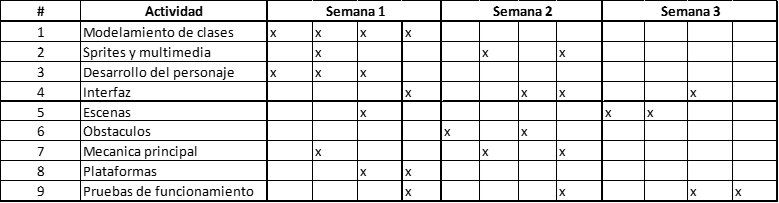
\includegraphics[width=10cm]{cronog.png}
    \centering
    \caption{Cronograma}
    \label{fig:Cronograma}
    \end{figure}
 
\end{document}